%================ch1======================================
\chapter{Introduction}\label{ch:ch1}

\section{Gaia Mission}
We have come a long way in observing the skies, from the naked eye to the mural instrument, from telescopes to space missions. The Gaia mission \citep{gaia} \citep{gaiafaccs} is one such astrometry mission launched in 2013. The spacecraft aims to measure the positions, distances and motions of celestial objects, not just in our galaxy but much beyond. The mission aims to be the most precise 3D catalogue of the sky, mapping every object it can while also measuring their motions which can give clues about the origin and evolution of our galaxy, the Milky Way.

The mission aims to determine the position and parallax of around a billion stars to an accuracy of around 20 $\mu as$. The catalogue is set to be released in stages. The first data release took place in 2016 \citep{gaiadr1}, based on 14 months of observation. It inlcuded the positions and magnitudes for over a billion stars using only Gaia data. The second data release took place in 2018 \citep{gaiadr2}, after 22 months of observations, and improved on the precision of the previous release, as well as adding parallaxes and proper motions.

\section{Star Clusters}
Gravity is one of the 4 fundamental forces which keeps large celestial structures in place. A star cluster is a gravitationally bound group of stars. They share a common origin and provide a way to study stellar evolution. They can be globular or open.

\subsection{Globular Clusters}
A globular cluster is a roughly spherical collection of stars orbiting the galactic core. They have a dense concentration of stars in their centers and are thinly spread out further from the center in the halo. They are composed of thousands of low metal stars. They are generally found in the halo of a galaxy and are generally older than the stars in open clusters. \citep{globclust} The proportion of metals, called metallicity, is rather low in these stars. The metallicity of a star is an indicator of its age, and the low metallicity of stars in globular clusters shows this. \citep{introstars}

\subsection{Open Clusters}
An open cluster is a group of a few thousand stars formed from the same molecular cloud. They are named so because often individual component stars can be resolved rather easily with a telescope. They are generally found in the disc of the galaxy. They are rather loosely bound by gravitational attraction between the member stars. Gravitational effects from other massive bodies as it moves on its journey around the center of the galaxy often disperse the order of these clusters. They are much younger compared to globular clusters, some even showing signs of nebulosity. Properties of the cluster members can be determined easily because they have are at the same distance away from us and they have a similar age and chemical composition \citep{openclust}. This will also be the focus of this report.

\section{Gaia Data for Open Clusters}
While the Gaia mission provided us with very precise data regarding astronomical objects, they are not classified. The study by Cantat-Gaudin et. al \citep{cg} aims to determine a list of members of open clusters and derive mean parameters from them using Gaia data. They obtained a list of 1229 open clusters with associated members and cluster parameters. The cluster members identified by Cantat-Gaudin are available on the VizieR database \citep{vizier}, which is used for this study. The data lists the positions of the clusters and their members, with parallaxes, proper motions and color magnitudes. From the other Gaia data, more information can be queried for individual stars. Combining the data, the properties of these star clusters can be studied. Eventually, we can separate the binary stars from the single ones and study their radial distributions. We can then examine their evolution and morphology.

\section{Photometry}
The art of measuring the electromagnetic radiation from a point source in the sky is known as photometry. Thus, we can use this information to calculate the distance to an object, its mass, its temperature and chemical composition. To determine some of these factors, we will plot a very useful graph known as a Hertzsprung-Russel chart or a color magnitude diagram.


\subsection{Color Magnitude Diagrams}
To study about the life cycles of stars, their evolution, we plot the luminosities of stars against their color. This is essentially a plot of the total energy given by a star against the surface temperature. This is known as a Hertzsprung-Russel diagram (HR diagram) or a color magnitude diagram (CMD). There are four major groups of stars in this plot. The smear in the bottom left representing the white dwarfs. They are among the older stars in the life cycle and most open clusters don't have them. They undergo hydrogen fusion and take up the bulk of a star's life. The horizontal branch breaking away from the main sequence corresponds to the red giant stars and the top right belongs to the supergiants. There are other minor divisions in the clusters, such as blue stragglers as well.  \citep{introstars}

\begin{figure}[H]
	\centering
	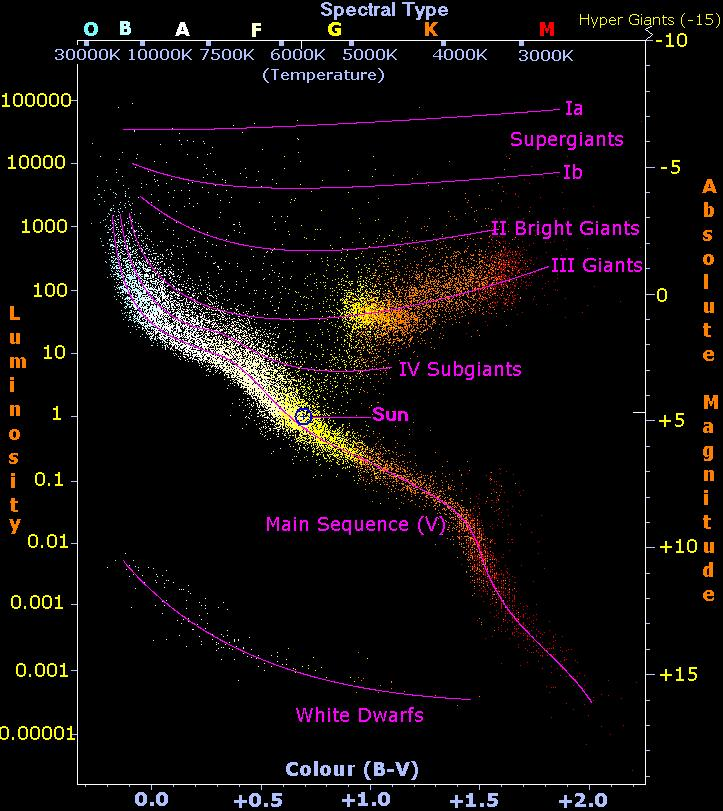
\includegraphics[width=0.6\linewidth]{hr-diagram.jpg}
	\caption{H-R Diagram \citep{wimecommons}}
	\label{fig:image1}
\end{figure}

\subsection{Isochrones}
A stellar isochrone is a curve on the color magnitude diagram indicating a population of stars of the same age. They can be used to date stars in open clusters because they all approximately have the same age. Isochrone data is available in the internet and they can be downloaded to test which one gives the best fit. The best fitting isochrones don't just reveal the age of the cluster, but much more information.



